\documentclass{beamer}
\mode<presentation> {
  \usetheme{Madrid} % or try Darmstadt, Madrid, Warsaw, ...
  \usecolortheme{default} % or try albatross, beaver, crane, ...
  \usefonttheme{default}  % or try serif, structurebold, ...
  \setbeamertemplate{navigation symbols}{}
  \setbeamertemplate{caption}[numbered]
} 

\usepackage[english]{babel}
\usepackage[utf8x]{inputenc}
\usepackage{graphicx}
\usepackage{amsmath}
\usepackage{amsfonts}
\usepackage{amssymb}
\usepackage{hyperref}

\usepackage{import}
\usepackage{standalone}
\usepackage{wrapfig}

\usepackage{tikz}
\usepackage{subcaption}
\usetikzlibrary{calc}
\usetikzlibrary {shapes.geometric}

%Defines theorem enviroments
\theoremstyle{definition}


\title[Tilling the Plane]{Tessellating the Plane: from periodic tilings to Hat and Spectre}
\author{Rory Yarr}
% \institute[University of Melbourne] % (optional)
% {
%    From periodic frieze groups, lattices and wallpaper groups to the aperiodic Hat and Spectre!
% }
\date{\today}

\begin{document}

\begin{frame}
  \titlepage

  \begin{abstract}
    From periodic frieze groups, lattices and wallpaper groups to the aperiodic Hat and Spectre!
  \end{abstract}
\end{frame}

\begin{frame}{Frize Groups}
    
\end{frame}


\begin{frame}{Wallpaper groups}
    \begin{figure}
        \centering
        % 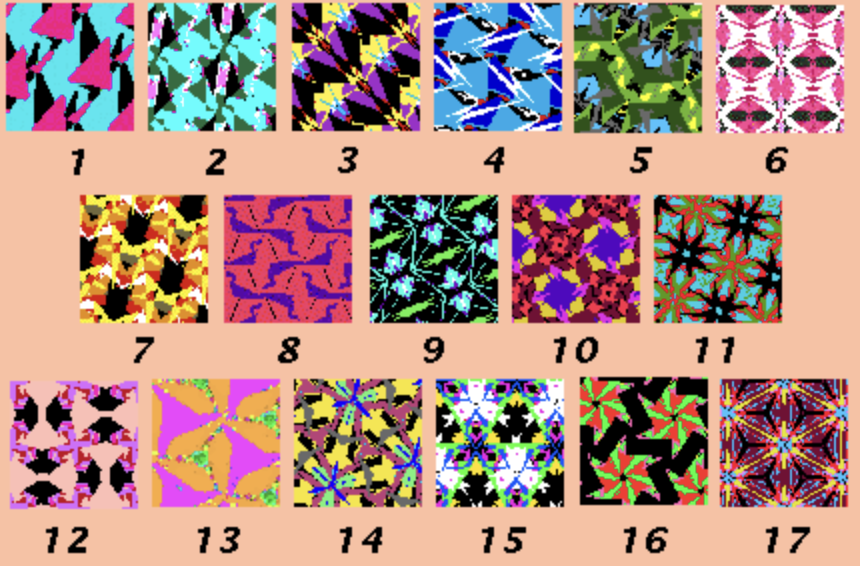
\includegraphics[width=0.9\textwidth]{Figures/WallpaperGroupsExample.png}
        \caption{The 17 wallpaper groups \cite{Clark1}}
        \label{fig:17WallpaperGroups}
    \end{figure}
\end{frame}


\begin{frame}{Hilbert problems}
    
\end{frame}

\begin{frame}{Penrose Tilling}
    
\end{frame}


\end{document}